\documentclass[portrait, final, a0paper, fontscale=0.277]{baposter}

\usepackage{calc}
\usepackage{graphicx}
\usepackage{amsmath}
\usepackage{amssymb}
\usepackage{relsize}
\usepackage{multirow}
\usepackage{rotating}
\usepackage{bm}
\usepackage{url}
\usepackage{footnote}
\usepackage{graphicx}
\usepackage{multicol}
\usepackage{palatino}
\usepackage[ruled,linesnumbered,noend]{algorithm2e}

\newcommand{\captionfont}{\footnotesize}

\graphicspath{{images/}{../images/}}

\newcommand{\HEART}{\textsc{HeaRTDroid}\xspace}
\newcommand{\OPENML}{\textsc{OpenML}\xspace}
\newcommand{\AUTOWEKA}{\textsc{Auto-WEKA}\xspace}
\newcommand{\WEKA}{\textsc{WEKA}\xspace}

\setlength{\columnsep}{1.5em}
\setlength{\columnseprule}{0mm}

\newcommand{\compresslist}{
\setlength{\itemsep}{1pt}
\setlength{\parskip}{0pt}
\setlength{\parsep}{0pt}
}

%%%%%%%%%%%%%%%%%%%%%%%%%%%%%%%%%%%%%%%%%%%%%%%%%%%%%%%%%%%%%%%%%%%%%%%%%%%%%%
\begin{document}

\definecolor{lightblue}{rgb}{0.145,0.6666,1}
\definecolor{lightorange}{rgb}{0.9,0.4,0}
\definecolor{lightgreen}{RGB}{93,179,77}

\hyphenation{resolution occlusions}
\begin{poster}
{
    % Show grid to help with alignment
    grid=false,
    % Column spacing
    colspacing=1em,
    % Color style
    bgColorOne=white,
    bgColorTwo=white,
    borderColor=lightblue,
    headerColorOne=black,
    headerColorTwo=lightblue,
    headerFontColor=white,
    boxColorOne=white,
    boxColorTwo=lightblue,
    % Format of textbox
    textborder=roundedleft,
    % Format of text header
    eyecatcher=true,
    headerborder=closed,
    headerheight=0.1\textheight,
    headershape=roundedright,
    headershade=shadelr,
    headerfont=\Large\bf\textsc, %Sans Serif
    textfont={\setlength{\parindent}{1.5em}},
    boxshade=plain,
    background=plain,
    linewidth=2pt
}
% Eye Catcher
{
\includegraphics[height=9em]{agh}}
% Title
{\bf\textsc{Concept of rule-based configurator for Auto-WEKA using OpenML}\vspace{0.5em}}
% Authors
{
    \textsc{Patryk Kiepas, Szymon Bobek, Grzegorz J. Nalepa
        \\ \texttt{\{kiepas,sbobek,gjn\}@agh.edu.pl}}
}

%%%%%%%%%%%%%%%%%%%%%%%%%%%%%%%%%%%%%%%%%%%%%%%%%%%%%%%%%%%%%%%%%%%%%%%%%%%%%%
\headerbox{Contribution}{name=contribution,column=0,row=0, span=3}{
%%%%%%%%%%%%%%%%%%%%%%%%%%%%%%%%%%%%%%%%%%%%%%%%%%%%%%%%%%%%%%%%%%%%%%%%%%%%%%
\noindent
In this poster we describe a mechanism for automatic recommendation of suitable machine learning algorithms and their parameters. This was achieved by use of \OPENML database and a rule-based configurator to make an recommendation. Created recommendations are then used to improve \AUTOWEKA tool by reducing its search space and in result its computational time \cite{autoweka2013}.

\vspace{0.3em}
}

%%%%%%%%%%%%%%%%%%%%%%%%%%%%%%%%%%%%%%%%%%%%%%%%%%%%%%%%%%%%%%%%%%%%%%%%%%%%%%
\headerbox{1.Knowledge acquisition}{name=acquisition,column=0,span=1,row=0,below=contribution}{
%%%%%%%%%%%%%%%%%%%%%%%%%%%%%%%%%%%%%%%%%%%%%%%%%%%%%%%%%%%%%%%%%%%%%%%%%%%%%%
\noindent
The initial phase is about creating a meta-knowledge that describes dependencies between datasets and performance of machine learning algorithms executed on them.

\vspace{-1em}
\centering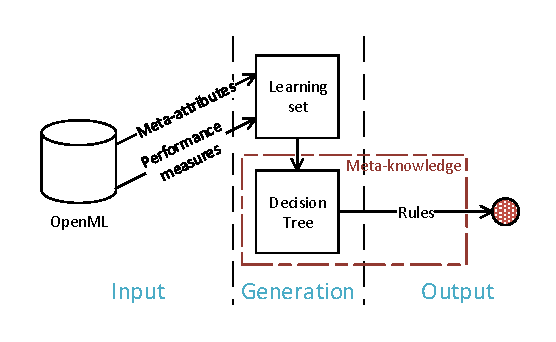
\includegraphics[width=1\textwidth]{flow_1}

\vspace{-1.5em}
\begin{itemize}
    \item Each dataset is described by meta-attributes (e.g. number of classes, attribute entropy)
    \item Missing meta-attributes are filled with Amelia-II algorithm \cite{amelia2011},
    \item Data about all meta-attributes with corresponding algorithms creates a learning set,
    \item Building meta-knowledge requires filtering OpenML database described by three parameters (shown in result section),
    \item Rules are extracted from decision tree created with J48 algorithm on the learning set.
\end{itemize}
}

%%%%%%%%%%%%%%%%%%%%%%%%%%%%%%%%%%%%%%%%%%%%%%%%%%%%%%%%%%%%%%%%%%%%%%%%%%%%%%
\headerbox{2. Recommendation}{name=recommendation,column=1,span=1,row=0,below=contribution}{
%%%%%%%%%%%%%%%%%%%%%%%%%%%%%%%%%%%%%%%%%%%%%%%%%%%%%%%%%%%%%%%%%%%%%%%%%%%%%%
\noindent
In second stage meta-attributes of each new dataset are matched with meta-knowledge in order to build a set consisting of suitable algorithms with their parameters.
\\
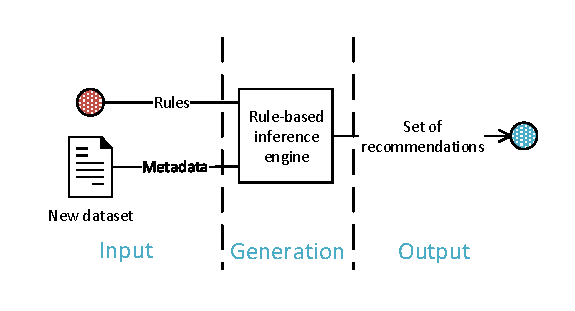
\includegraphics[width=1\textwidth]{flow_2}
\begin{itemize}
    \item Configurator is a rule-based inference engine in \HEART\footnote{http://bitbucket.org/sbobek/heartdroid} implementation,
    \item Inference engine works in fixed-order inference mode,
    \item Size of set of recommendations depends on number of fired rules by configurator,
    \item Recommended parameters are fixed within recommended algorithm,
    \item This phase requires single instance of meta-knowledge.
\end{itemize}
\vspace{0.04em}
}

%%%%%%%%%%%%%%%%%%%%%%%%%%%%%%%%%%%%%%%%%%%%%%%%%%%%%%%%%%%%%%%%%%%%%%%%%%%%%%
\headerbox{3. Tuning}{name=tuning,column=2,span=1,row=0,below=contribution}{
%%%%%%%%%%%%%%%%%%%%%%%%%%%%%%%%%%%%%%%%%%%%%%%%%%%%%%%%%%%%%%%%%%%%%%%%%%%%%%
\noindent
Tuning phase uses created set of recommendation to reduce search space in hyper-optimization process done by \AUTOWEKA tool.
\\
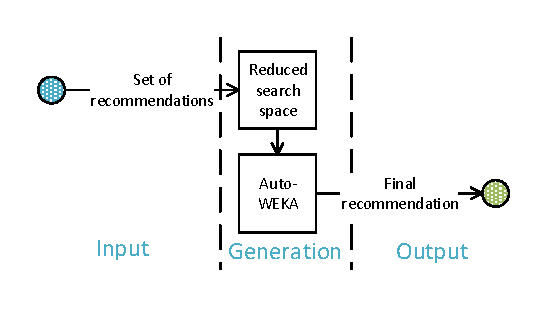
\includegraphics[width=1\textwidth]{flow_3}
\begin{itemize}
    \item \AUTOWEKA's search space is reduced to recommended algorithms,
    \item New experiment is prepared with use of BATCH file where list of algorithms to consider and its parameter ranges is storage,
    \item Output of this phase is a final recommendation consisting of single algorithm with parameters,
    \item Final recommendation is a result of \AUTOWEKA's hyper-parameter optimization,
    \item Output recommendation can be used directly in \WEKA tool.
\end{itemize}
}

%%%%%%%%%%%%%%%%%%%%%%%%%%%%%%%%%%%%%%%%%%%%%%%%%%%%%%%%%%%%%%%%%%%%%%%%%%%%%%
\headerbox{Results}{name=results,column=0,span=3,below=tuning}{
%%%%%%%%%%%%%%%%%%%%%%%%%%%%%%%%%%%%%%%%%%%%%%%%%%%%%%%%%%%%%%%%%%%%%%%%%%%%%%
\begin{minipage}{0.35\textwidth}
    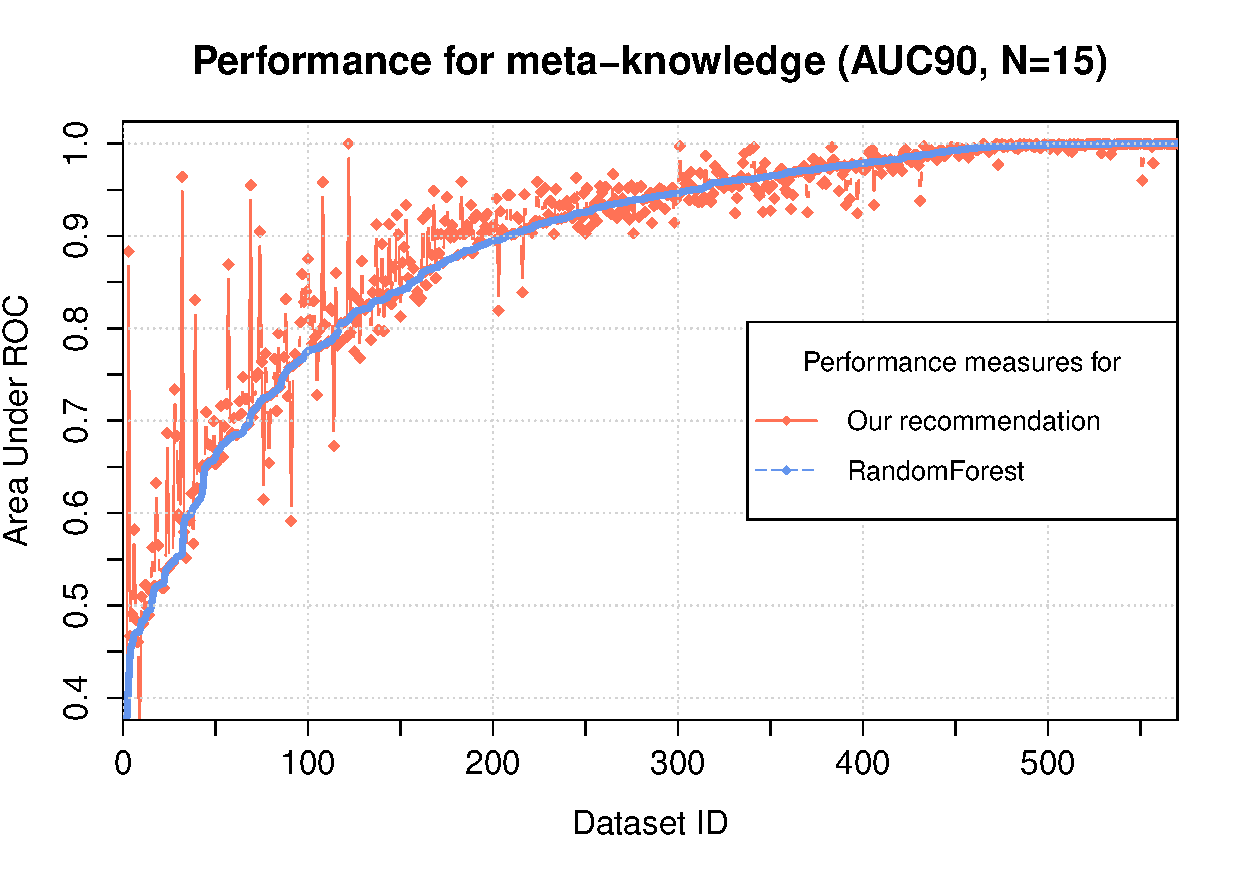
\includegraphics[width=1\textwidth]{auc90_C15_A5}
\end{minipage}\hfill
\begin{minipage}{0.62\textwidth}
    \begin{itemize}
        \item Results represents difference in performance of our recommendation for 570 test datasets against performance of \textit{state-of-the-art} algorithm -- \textsc{RandomForest},
        \item In order to test our system and not \AUTOWEKA tool we analyse best recommendations made during second stage,
        \item Meta-knowledge for this experiment was created with parameters:
        \begin{itemize}
            \item Selected performance measures: $area~under~ROC >= 0.9$,
            \item Number of algorithm to consider: $15$ most used algorithms from \OPENML,
            \item Using meta-attributes with less than $20\%$ missing values.
        \end{itemize}
        \item Results are visibly good where \textsc{RandomForest} is doing poorly (datasets 1-250).
    \end{itemize}
\end{minipage}\hfill
}

%%%%%%%%%%%%%%%%%%%%%%%%%%%%%%%%%%%%%%%%%%%%%%%%%%%%%%%%%%%%%%%%%%%%%%%%%%%%%%
\headerbox{Future work}{name=future,column=0,span=2,above=bottom}{
%%%%%%%%%%%%%%%%%%%%%%%%%%%%%%%%%%%%%%%%%%%%%%%%%%%%%%%%%%%%%%%%%%%%%%%%%%%%%%
\vspace{0.25em}
\begin{itemize}
    \item Learning and gaining additional meta-knowledge during recommendation phase,
    \item Improving rules induction from the learning set,
    \item Adding parameter recommendation in form of value ranges,
    \item Adding guidance for data preprocessing methods,
    \item Including more data sources (e.g. MLComp portal, hand-crafted rules),
    \item Using synthetic datasets for better coverage of meta-attributes space.
\end{itemize}
}

%%%%%%%%%%%%%%%%%%%%%%%%%%%%%%%%%%%%%%%%%%%%%%%%%%%%%%%%%%%%%%%%%%%%%%%%%%%%%%
\headerbox{References}{name=references,column=2,above=bottom}{
%%%%%%%%%%%%%%%%%%%%%%%%%%%%%%%%%%%%%%%%%%%%%%%%%%%%%%%%%%%%%%%%%%%%%%%%%%%%%%
\vspace{0.35em}

\smaller
\bibliographystyle{ieee}
\renewcommand{\section}[2]{\vskip 0.05em}
\begin{thebibliography}{1}\itemsep=-0.01em
    \setlength{\baselineskip}{0.4em}
    \bibitem{autoweka2013}
    Thornton, C., Hutter, F., Hoos, H., Leyton-Brown, K.: Auto-WEKA: Combined selection and hyperparameter optimization of classification algorithms. In: Proc. of KDD-2013. pp. 847--855 (2013)

    \bibitem{amelia2011}
    Honaker, J., King, G., Blackwell, M.: Amelia II: A program for missing data. Journal of Statistical Software 45(7), 1--47 (12 2011), http://www.jstatsoft.org/v45/i07

    \bibitem{brazdil2008}
    Brazdil, P., Giraud-Carrier, C., Soares, C., Vilalta, R.: Meta-learning: Concepts and techniques. In: Metalearning: Applications to Data Mining. Springer Publishing Company, Incorporated, 1 edn. (2008)
\end{thebibliography}
}

\end{poster}

\end{document}
